\documentclass[11pt,a4paper]{article}

% ---------------------------------------------------------------- packages
\usepackage[T1]{fontenc}
\usepackage[utf8]{inputenc}
\usepackage{libertinus}
\usepackage[scaled=0.86]{sourcecodepro}
\usepackage[margin=2.1cm,top=2.2cm,bottom=2.2cm]{geometry}
\usepackage{amsmath,amssymb}
\usepackage{booktabs}
\usepackage{array}
\usepackage{xcolor}
\usepackage{graphicx}
\usepackage{enumitem}
\usepackage{titlesec}
\usepackage{tcolorbox}
\usepackage{microtype}
\usepackage{caption}
\usepackage{fancyhdr}
\usepackage[hidelinks,colorlinks=true,linkcolor=accent,urlcolor=accent]{hyperref}
\tcbuselibrary{skins,breakable}

% ------------------------------------------------------------------ colours
\definecolor{accent}{HTML}{2A78D6}
\definecolor{accent2}{HTML}{EB6834}
\definecolor{aqua}{HTML}{1BAF7A}
\definecolor{ink}{HTML}{0B0B0B}
\definecolor{ink2}{HTML}{52514E}
\definecolor{ink3}{HTML}{8A8983}
\definecolor{rule}{HTML}{E3E2DD}
\definecolor{surf2}{HTML}{F3F2EF}

% ------------------------------------------------------------------ styling
\titleformat{\section}{\normalfont\large\bfseries\color{accent}}{\thesection}{0.6em}{}
\titleformat{\subsection}{\normalfont\normalsize\bfseries\color{ink}}{\thesubsection}{0.55em}{}
\titlespacing*{\section}{0pt}{1.2em}{0.45em}
\titlespacing*{\subsection}{0pt}{0.85em}{0.3em}

\captionsetup{font=small,labelfont={bf,color=accent},textfont={color=ink2}}
\captionsetup{justification=raggedright,singlelinecheck=false}
\renewcommand{\arraystretch}{1.16}
\setlength{\parindent}{0pt}
\setlength{\parskip}{0.42em}
\sloppy
\setlength{\emergencystretch}{3em}

\pagestyle{fancy}
\fancyhf{}
\renewcommand{\headrulewidth}{0.4pt}
\renewcommand{\headrule}{\hbox to\headwidth{\color{rule}\leaders\hrule height \headrulewidth\hfill}}
\fancyhead[L]{\small\color{ink3}Recovering drift fields from random walks}
\fancyfoot[C]{\small\color{ink3}\thepage}

\newtcolorbox{keybox}[1][]{
  enhanced, breakable, colback=accent!5, colframe=accent, boxrule=0pt,
  leftrule=2.5pt, arc=0pt, left=8pt, right=8pt, top=5pt, bottom=5pt, #1
}
\newtcolorbox{warnbox}[1][]{
  enhanced, breakable, colback=accent2!6, colframe=accent2, boxrule=0pt,
  leftrule=2.5pt, arc=0pt, left=8pt, right=8pt, top=5pt, bottom=5pt, #1
}
% a framed, titled box for every training objective, so the losses stand out
\newtcolorbox{lossbox}[1]{
  enhanced, breakable, colback=surf2, colframe=ink3, boxrule=0.4pt, arc=1.5pt,
  left=8pt, right=8pt, top=4pt, bottom=4pt,
  title={\small\bfseries #1}, coltitle=ink, colbacktitle=rule,
  toptitle=1.5pt, bottomtitle=1.5pt
}

\newcommand{\code}[1]{{\ttfamily\small #1}}
\newcolumntype{L}[1]{>{\raggedright\arraybackslash}p{#1}}
\newcommand{\dt}{\Delta t}
\newcommand{\dx}{\Delta x}
\newcommand{\E}{\mathbb{E}}
\newcommand{\rss}{\rho_{\mathrm{ss}}}

% ==========================================================================
\begin{document}

\begin{center}
{\LARGE\bfseries\color{ink} Recovering drift fields from random walks}\\[0.3em]
{\large\color{accent} Six estimators, one set of walkers, and where each one wins}\\[0.8em]
{\color{ink3}\small The \code{dfi} package \quad\textbullet\quad 46 tests (45 pass, 1 skips) \quad\textbullet\quad
every number reproduced by a numbered script}
\end{center}

\vspace{0.2em}\hrule height 0.4pt \vspace{0.8em}

\begin{keybox}
\textbf{The question.} Particles move by $\mathrm dx = b(x)\,\mathrm dt+\sqrt{2D}\,\mathrm dW$.
From their observed motion, recover the vector field $b$. Over one recorded step the random
displacement is about 30 times the drift displacement (about 1000 times in power), so every
method is an exercise in averaging away a much larger random term without averaging away
the field.

\textbf{What was built.} A simulator, six estimators of increasing structure, and one
measurement protocol that runs all of them on the \emph{same} walkers, so that differences
are differences between methods and not between experiments.

\textbf{Three results.} (i) A network trained across many simulated fields beats every
classical estimator by roughly 25\textendash40\% \textemdash{} and loses to the simplest kernel on
fields from a generator it never saw. (ii) At equilibrium, \emph{static positions} carry more
about the drift than the increments do, decisively so in 5D. (iii) Static positions are
\emph{exactly} blind to circulation: adding a rotating component to the drift leaves every
snapshot-based estimate unchanged to the last bit.
\end{keybox}

% ==========================================================================
\section{The problem}

\subsection{The dynamics}

The overdamped Langevin equation
\begin{equation}
  \mathrm dx \;=\; b(x)\,\mathrm dt \;+\; \sqrt{2D}\,\mathrm dW
  \label{eq:sde}
\end{equation}
models a particle in a force field $b$ with thermal agitation of strength $D$ (the
diffusion coefficient). $W$ is a $d$-dimensional Wiener process (Brownian motion): its
increments over disjoint time intervals are independent and Gaussian, with
\begin{equation}
  \E[\mathrm dW_i] = 0,
  \qquad
  \E[\mathrm dW_i\,\mathrm dW_j] = \delta_{ij}\,\mathrm dt ,
  \qquad\text{i.e.}\qquad
  W(t+\dt)-W(t)\;\sim\;\mathcal N(0,\ \dt\, I_d).
\end{equation}
The noise term $\sqrt{2D}\,\mathrm dW$ therefore has zero mean and variance $2D\,\mathrm dt$
per component; for $b=0$ this is free diffusion with mean squared displacement $2dDt$.
Its standard deviation grows like $\sqrt{\mathrm dt}$, much faster than the drift's
$\mathrm dt$ for small $\mathrm dt$ \textemdash{} which is the whole difficulty below.

The inverse problem, recovering $b$ from observed motion, appears in single-particle
tracking, active matter, ecology, and anywhere a stochastic differential equation is fitted
to a trajectory. Two kinds of data support two fundamentally different answers.

\subsection{Trajectories: the drift is a conditional mean}

Positions recorded in time order at spacing $\dt$. Integrating \eqref{eq:sde} over one step,
$\dx = b(x)\dt + \sqrt{2D}\,\Delta W + O(\dt^{3/2})$, so
\begin{equation}
  \E[\dx \,|\, x] = b(x)\,\dt + O(\dt^2),
  \qquad
  \mathrm{Cov}[\dx \,|\, x] = 2D\dt\, I + O(\dt^2).
\end{equation}
This is the Kramers\textendash Moyal relation. It turns each recorded step into a noisy
sample of the field at the point the step started from:
\begin{equation}
  y_i \;\equiv\; \frac{\dx_i}{\dt} \;=\; b(x_i) + \eta_i ,
  \qquad
  \eta_i \sim \mathcal N\!\Big(0,\ \frac{2D}{\dt}\, I\Big).
  \label{eq:km}
\end{equation}
Estimating $b$ is therefore a regression of $y$ on $x$. The noise $\eta$ grows as $\dt$
shrinks: in the 2D settings used here ($D=0.3$, $\dt\approx10^{-3}$, RMS$|b|\approx1$) its
magnitude is 32 times the drift's. The six estimators differ only in how they pool
neighbouring samples to beat it down.

\subsection{Snapshots: what the stationary density can and cannot tell}

Positions \emph{without} time order, drawn from the stationary density $\rss$. The density
obeys the Fokker\textendash Planck equation
\begin{equation}
  \partial_t \rho = -\nabla\!\cdot J,
  \qquad
  J = b\,\rho - D\nabla\rho ,
\end{equation}
where $J$ is the probability current. In the stationary state $\nabla\!\cdot J_{\mathrm{ss}}=0$.
Solving the definition of $J$ for $b$ gives an identity valid for \emph{any} drift:
\begin{equation}
  b \;=\; \underbrace{D\,\nabla\log\rss}_{\text{visible in snapshots}}
  \;+\; \underbrace{J_{\mathrm{ss}}/\rss}_{\text{invisible in snapshots}} .
  \label{eq:split}
\end{equation}
Snapshots determine $\rss$, hence the first term (the \emph{score} $\nabla\log\rss$, times
$D$). They say nothing about the second: any field $c$ with $\nabla\!\cdot(c\,\rss)=0$ can be
added to $b$ without changing $\rss$, so infinitely many drifts produce the same snapshots.
Only when the current vanishes \textemdash{} \emph{detailed balance}, i.e.\ thermodynamic
equilibrium \textemdash{} is $b = D\nabla\log\rss$ a pure gradient, fully determined by
positions alone.

\textbf{The fields used here make this exact.} Every drift is built as
\begin{equation}
  b = -\nabla U + \omega\, A\nabla U ,
  \qquad A^\top = -A ,
  \label{eq:field}
\end{equation}
from one scalar potential $U$. Substituting $\rss = e^{-U/D}/Z$ into the current gives
$J_{\mathrm{ss}} = \omega\,\rss\, A\nabla U$, and its divergence vanishes term by term:
$\nabla\!\cdot(A\nabla U) = A_{ij}\partial_i\partial_j U = 0$ (an antisymmetric matrix
contracted with a symmetric Hessian), and $\nabla U\!\cdot\! A\nabla U = 0$ (an antisymmetric
quadratic form). So $\rss\propto e^{-U/D}$ for \emph{every} $\omega$: the rotational part
$\omega A\nabla U$ drives a steady circulating current $J_{\mathrm{ss}}\neq0$ yet leaves the
density untouched, and the score recovers only the gradient part,
\begin{equation}
  D\,\nabla\log\rss \;=\; -\nabla U \;=\; b_{\mathrm{grad}} .
  \label{eq:score}
\end{equation}

\begin{figure}[h]
\centering
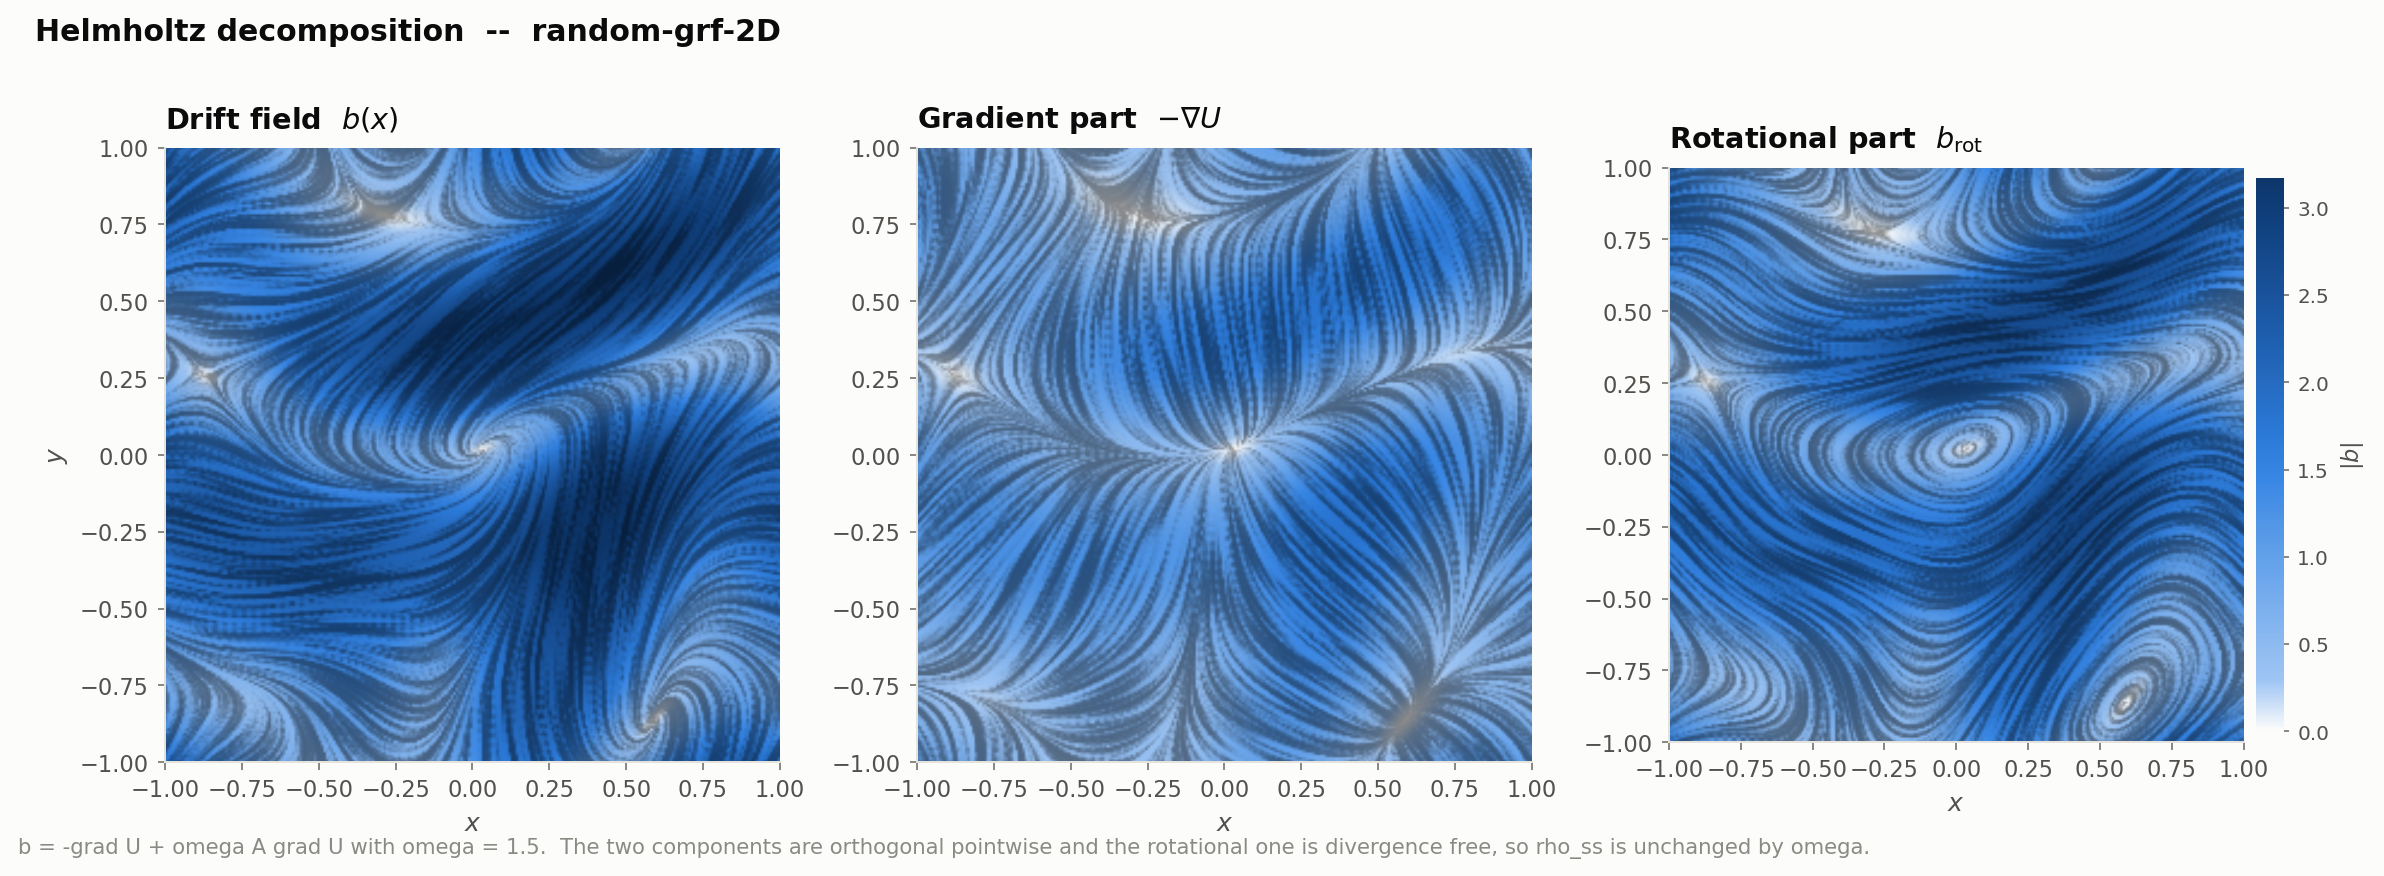
\includegraphics[width=\textwidth]{figs/helmholtz.png}
\caption{A drift field \eqref{eq:field} and its two parts. The rotational part (right) is
divergence-free and everywhere orthogonal to $\nabla\rss$, so $\rss$ is identical for every
$\omega$: a snapshot dataset cannot distinguish a system with no circulation from one with a
great deal of it.}
\end{figure}

\begin{warnbox}
\textbf{The identifiability gap is a property of the data, not of the estimators.} From
snapshots, only the gradient part of $b$ is recoverable, whatever the method; from
trajectories, all of $b$ is. The comparisons below are read with this limitation in mind.
\end{warnbox}

% ==========================================================================
\section{Setup and measurement protocol}

\textbf{Fields.} $U$ is a Gaussian random field on the torus $[-1,1]^d$ with a tunable
correlation length, and $b$ is built from it by \eqref{eq:field}, so $\omega$ dials
circulation without touching $\rss$. Six other generators (sparse wells, cellular band-pass
patterns, Perlin noise, power-law spectra, terraces, an egg-carton lattice) are used only to
test generalisation.

\textbf{Simulation.} Euler\textendash Maruyama with sub-stepping: the integrator runs at
$\dt/\text{substeps}$ while positions are recorded at $\dt$, so that an $O(\dt)$ bias in an
estimator is not confused with an $O(\dt)$ error of the integrator. Trajectories are cached
by configuration, so every estimator sees bit-identical walkers.

\begin{figure}[h]
\centering
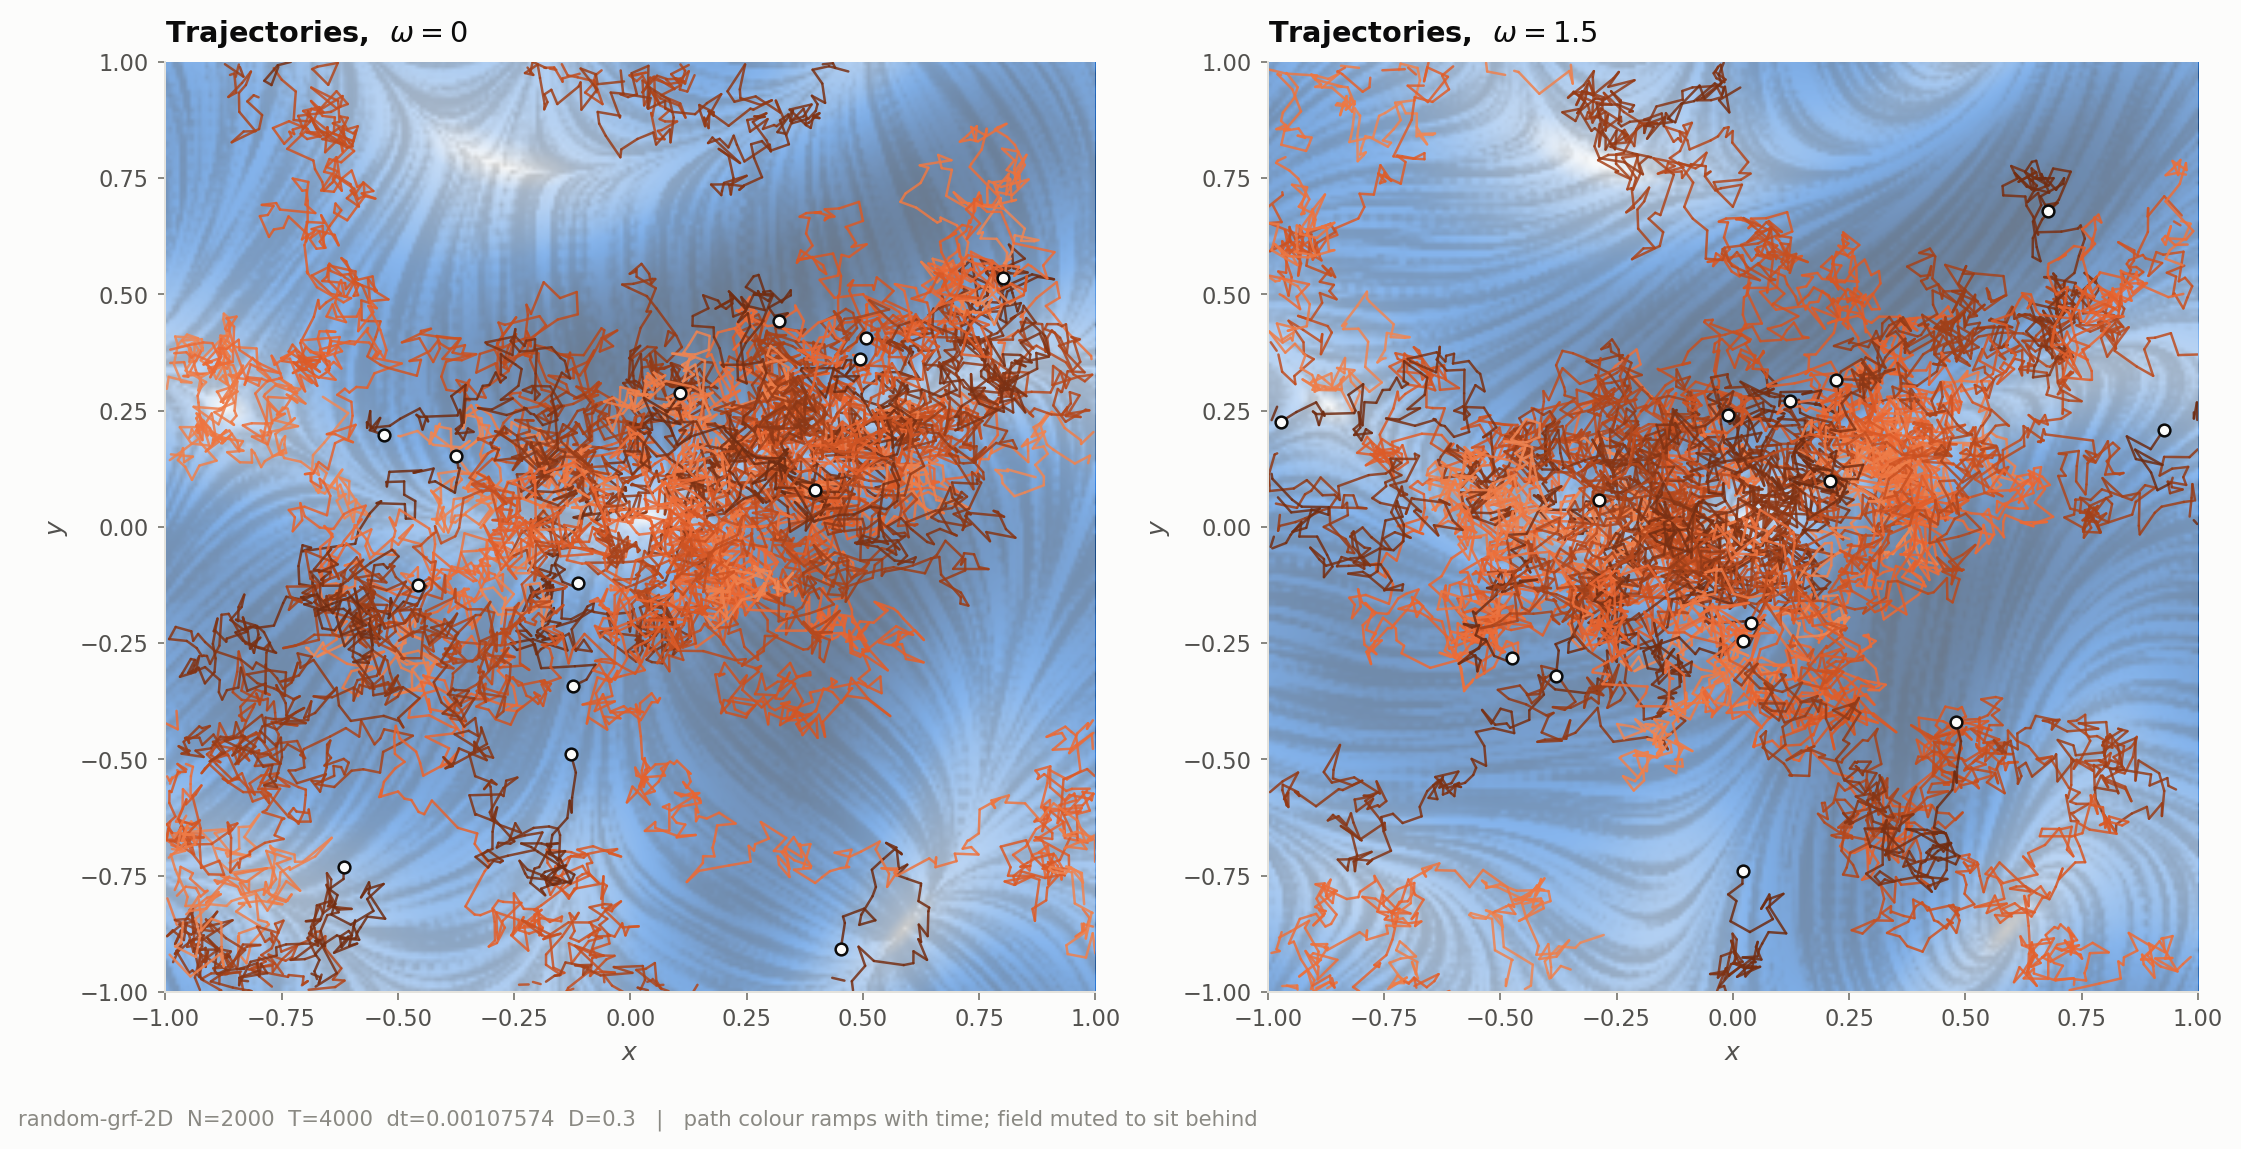
\includegraphics[width=0.88\textwidth]{figs/trajectories.png}
\caption{What the estimators are given: 2000 walkers $\times$ 4000 steps in the same field,
without and with circulation ($\omega=0$ and $1.5$), paths coloured by time. The drift is
invisible in any single step and appears only after averaging thousands of them. The
circulation on the right is recoverable from the increments and, by \eqref{eq:split},
absent from the positions.}
\end{figure}

\textbf{Error metric.} Every estimate is scored against the true field at $n=20\,000$
points $x_j$ drawn from $\rss$ \textemdash{} where the walkers actually go, and so where the
estimate will be used:
\begin{equation}
  \mathrm{nrmse}
  \;=\; \left(\frac{\sum_j |\hat b(x_j) - b(x_j)|^2}{\sum_j |b(x_j)|^2}\right)^{1/2} .
  \label{eq:nrmse}
\end{equation}
It is 0 for a perfect estimate and exactly 1 for the trivial estimate $\hat b\equiv0$, so
$0.10$ means ``wrong by 10\% of the field's typical magnitude'', and anything near 1 means
the method has learned essentially nothing. Lower is better.

\textbf{Tuning.} Every method chooses its own smoothing (bin size, bandwidth, basis size,
training length) by cross-validation grouped \emph{by walker}, never by sample. Splitting
increments at random lets a held-out point sit one time step away from its training
neighbours, and the criterion then rewards a smoothing scale far too small (§\ref{sec:selftuning}).

% ==========================================================================
\section{Six estimators, from simplest to most structured}

\begin{center}
\small
\begin{tabular}{@{}rL{0.25\textwidth}L{0.21\textwidth}L{0.40\textwidth}@{}}
\toprule
& \textbf{method} & \textbf{data} & \textbf{what it assumes} \\
\midrule
1 & binned Kramers\textendash Moyal & increments & $b$ is constant inside a cell \\
2 & kernel regression (Nadaraya\textendash Watson, local-linear) & increments & $b$ is smooth on one length scale \\
3 & basis projection (SFI) & increments & $b$ lies in a Fourier basis \\
4 & neural network (MLP, CNN) fitted to one dataset & increments & smoothness from architecture + early stopping \\
4b & amortised CNN, trained across 3000 fields & increments, binned & \textbf{what fields from this generator look like} \\
5 & KDE score, denoising score matching & positions only, plus $D$ & \textbf{equilibrium} (gradient drift) \\
\bottomrule
\end{tabular}
\end{center}

\subsection{Methods 1\textendash4: least squares on the increments}

All four trajectory estimators minimise the same squared loss over different classes of
functions. That loss is not an arbitrary choice; three properties make it the right one.

\begin{enumerate}[leftmargin=1.4em,itemsep=0.15em]
\item \textbf{It targets $b$ without seeing $b$.} Since $\E[\eta\,|\,x]=0$, for any candidate
      $f$
      \begin{equation}
        \E\,|y - f(x)|^2 \;=\; \E\,|b(x)-f(x)|^2 \;+\; \E\,|\eta|^2 ,
        \label{eq:decomp}
      \end{equation}
      the error against the unknown field plus a constant. Minimising the loss on the
      observed $y$ minimises the error against $b$; its minimiser over all functions is the
      conditional mean $\E[y\,|\,x]=b(x)$.
\item \textbf{It is maximum likelihood.} The Euler transition density is Gaussian,
      $p(x_{k+1}|x_k)\propto\exp\!\big(-|\dx_k-b(x_k)\dt|^2/4D\dt\big)$, so the
      log-likelihood of a trajectory is $-\frac{\dt}{4D}\sum_k|y_k-b(x_k)|^2+\text{const}$.
\item \textbf{It has a readable training curve.} Because the noise term in \eqref{eq:decomp}
      is about 1000 times the signal, the raw loss barely moves. The \emph{gain over predicting
      zero}, $L(0)-L(f) = \E|b|^2-\E|b-f|^2 = (1-\mathrm{nrmse}^2)\,\E|b|^2$, isolates the
      part that does.
\end{enumerate}

\begin{lossbox}{Losses of methods 1\textendash4 (data $\{(x_i,y_i)\}_{i=1}^n$, $y_i=\dx_i/\dt$)}
\vspace{-0.6em}
\begin{align*}
\text{1. binning:}\quad
  & \hat b_c = \arg\min_{\beta}\ \sum_{i:\,x_i\in c}|y_i-\beta|^2
    \ =\ \text{mean of the $y_i$ in cell $c$} \\
\text{2. kernel (NW):}\quad
  & \hat b(x) = \arg\min_{\beta}\ \sum_i K_h(x_i-x)\,|y_i-\beta|^2 \\
\text{2. kernel (local-linear):}\quad
  & (\hat b(x),\hat B) = \arg\min_{\beta,B}\ \sum_i K_h(x_i-x)\,|y_i-\beta-B(x_i-x)|^2 \\
\text{3. SFI:}\quad
  & \hat c = \arg\min_{c}\ \sum_i \Big|y_i-\sum_{|k|\le K} c_k\,\phi_k(x_i)\Big|^2,
    \qquad \hat b=\textstyle\sum_k \hat c_k\phi_k \\
\text{4. neural network:}\quad
  & \hat\theta = \arg\min_{\theta}\ \frac1n\sum_i |y_i-f_\theta(x_i)|^2
\end{align*}
\vspace{-1.1em}

$K_h$ is a Gaussian kernel of bandwidth $h$; $\phi_k$ are Fourier modes on the torus. The
smoothing parameter of each \textemdash{} cell width, $h$, the number of modes $K$, the number
of training steps \textemdash{} is chosen by the same squared loss on held-out walkers.
\end{lossbox}

Binning returns one value for the whole cell; the local-linear kernel removes the
first-order bias this carries; SFI (stochastic force inference) projects onto a global
Fourier basis, which is exactly the right basis for these fields. The networks are an MLP
with periodic input features, or a CNN that outputs the field on a grid; for the CNN the
loss over millions of increments reduces exactly to a few lattice statistics, so it is
trained full-batch with no sampling noise.

\subsection{Method 4b: an amortised network, trained across fields}

The per-dataset network must be refitted for every new dataset. The amortised one is trained
\emph{once} on simulated data and then only applied.

\textbf{Training data.} 3000 fields drawn from the generator with randomised parameters
(correlation length 0.3\textendash0.7; $\omega=0$ for half, otherwise in $[-1.5,1.5]$; $D$
log-uniform in $[0.05,1.5]$; 256 or 1024 walkers for 1000\textendash4000 steps). Each
dataset is summarised on a $64\times64$ lattice by the count $N_c$ and the summed increments
$Y_c=\sum_{i\in c}y_i$ per cell.

\textbf{Inputs.} Five channels built from $N_c$, $Y_c$ and the noise level
$\sigma^2=2D/\dt$, which is estimated from the data itself: a z-score $Y/(\sigma\sqrt N)$, a
shrunk mean $Y/(N+\lambda)$, and the data weight $N/(N+\lambda)$, with $\lambda=\sigma^2/\tau^2$.
The shrunk mean is precisely the per-cell Bayesian estimate: if a cell's mean increment
$\bar Y=Y/N\sim\mathcal N(b,\sigma^2/N)$ and the prior is $b\sim\mathcal N(0,\tau^2)$, the
posterior mean is $Y/(N+\lambda)$. The network starts from that and learns the spatial
coupling between cells.

\begin{lossbox}{Loss of method 4b (over training fields $m$, on the $64^2$ lattice nodes $c$)}
\vspace{-0.4em}
\[
  L(\theta) \;=\; \E_m\left[\
  \frac{\sum_c w_c\,\big|f_\theta(X^{(m)})_c - b^{(m)}_c\big|^2}
       {\sum_c w_c\,\big|b^{(m)}_c\big|^2}\ \right],
  \qquad w_c = 0.8\,\rss(c)/\bar\rho + 0.2 .
\]
\vspace{-0.9em}

$X^{(m)}$ are the input channels of training dataset $m$ and $b^{(m)}$ its true field.
Unlike every other method, the truth appears in this loss \textemdash{} but only for the
simulated training fields. On a new dataset the network is applied without retraining
and never sees $b$.
\end{lossbox}

\textbf{Why this loss.} The minimiser of $\E\,\|f(X)-b\|^2$ over all functions is the
posterior mean $\E[b\,|\,X]$ under the training distribution: the network is trained to be
the \emph{Bayes-optimal} estimator for fields drawn from its generator. That single fact
explains both its advantage and its failure mode (§\ref{sec:amort}). Dividing by
$\sum_c w_c|b_c|^2$ makes every field count equally regardless of its amplitude; weighting
by $\rss$ matches the evaluation metric \eqref{eq:nrmse}, with a 20\% floor so sparsely
visited regions are not ignored. The network is a periodic U-Net with no normalisation layers
(which would erase the physical amplitude), trained with the 8 symmetries of the square
lattice applied to inputs and outputs, vector components included.

\subsection{Method 5: the score, from static positions}

By \eqref{eq:score}, at equilibrium $b = D\,s$ with $s=\nabla\log\rss$. Estimating a score
from samples is exactly what training a diffusion model does.

\begin{lossbox}{Losses of method 5 (data: positions $\{x_i\}$ drawn from $\rss$)}
\vspace{-0.4em}
\begin{align*}
\text{denoising score matching:}\quad
  & L(\theta) = \E_{x,\ \sigma,\ \varepsilon}\
    \big|\,\sigma\, s_\theta(x+\sigma\varepsilon,\ \sigma) + \varepsilon\,\big|^2 \\
  & \qquad x\sim\text{data},\quad \varepsilon\sim\mathcal N(0,I),\quad
    \log\sigma\sim\mathcal U[\log 0.01,\ \log 0.5] \\
\text{KDE score:}\quad
  & s_h(x) = \nabla\log\hat\rho_h(x),
    \qquad \hat\rho_h(x)=\frac1n\sum_i \mathcal N(x;\,x_i,\,h^2 I) \\
\text{selection (both):}\quad
  & J(s) = \E_{x\sim\rss}\Big[\tfrac12|s(x)|^2 + \nabla\!\cdot s(x)\Big]
    \ \text{ on held-out positions}
\end{align*}
\vspace{-1.2em}
\end{lossbox}

\textbf{Why these losses.} Denoising score matching is again least squares onto a
conditional mean. For a noised point $\tilde x = x+\sigma\varepsilon$, Tweedie's formula gives
$-\E[\varepsilon\,|\,\tilde x]/\sigma = \nabla\log\rho_\sigma(\tilde x)$, where
$\rho_\sigma=\rss*\mathcal N(0,\sigma^2 I)$; so the minimiser of $L$ is the score of a
slightly blurred density, and $\sigma$ plays the role of a bandwidth. The selection criterion
$J$ (Hyv\"arinen score matching) satisfies, after an integration by parts with no boundary
terms on the torus, $J(s)=\tfrac12\E|s-\nabla\log\rss|^2+\text{const}$: it ranks candidate
scores by their true error using samples alone. It sets the KDE bandwidth $h$ and the noise
level $\sigma$ at which the trained network is read out.

% ==========================================================================
\section{Results}

\textbf{How to read Table~\ref{tab:main}.} Each entry is the nrmse \eqref{eq:nrmse}: 0 is
perfect, 1 is what predicting $\hat b\equiv0$ scores. The first column is the reference
configuration; each other column changes one thing, stated in the second header row, and the
third row gives the data budget in recorded transitions. Trajectory and snapshot rows are
different kinds of data on the same systems: the snapshot methods get independent positions
matched in number to the transitions (capped at 500k), plus the true $D$. Bold marks the best
method of each family in each column.

\begin{table}[t]
\caption{Normalised error \eqref{eq:nrmse} of every method; lower is better.}
\label{tab:main}
\centering
\small
\setlength{\tabcolsep}{4.2pt}
\begin{tabular}{@{}lrrrrrrr@{}}
\toprule
& \textbf{reference} & \shortstack[r]{\textbf{few}\\\textbf{walkers}}
& \shortstack[r]{\textbf{many}\\\textbf{walkers}} & \shortstack[r]{\textbf{strong}\\\textbf{noise}}
& \shortstack[r]{\textbf{position}\\\textbf{error}} & \textbf{3D} & \textbf{5D} \\
{\footnotesize changed}
& {\footnotesize 2D, $D=0.3$} & {\footnotesize 16 walkers} & {\footnotesize 1024 walkers}
& {\footnotesize $D=1.0$} & {\footnotesize $\sigma_{\mathrm{obs}}=0.02$} & {\footnotesize $d=3$} & {\footnotesize $d=5$} \\
{\footnotesize budget}
& {\footnotesize 4.8M} & {\footnotesize 192k} & {\footnotesize 12.3M}
& {\footnotesize 4.8M} & {\footnotesize 1.0M} & {\footnotesize 6.1M} & {\footnotesize 6.1M} \\
\midrule
\multicolumn{8}{@{}l}{\footnotesize\itshape trajectory methods \textemdash{} positions in time order} \\
1\ \ binned Kramers\textendash Moyal & 0.293 & 0.648 & 0.224 & 0.785 & 1.56 & 0.564 & 1.62 \\
2\ \ local-linear kernel & 0.126 & 0.358 & 0.088 & 0.280 & 1.25 & 0.261 & \textbf{0.925} \\
3\ \ SFI (Fourier basis) & 0.097 & 0.392 & 0.053 & 0.211 & 1.43 & \textbf{0.195} & 0.946 \\
4\ \ MLP & 0.100 & 0.340 & 0.080 & 0.319 & 1.38 & 0.223 & 0.927 \\
4\ \ CNN (one dataset) & 0.115 & 0.380 & 0.068 & 0.333 & 1.44 & 0.224 & \textemdash \\
4b amortised CNN & \textbf{0.060} & \textbf{0.257} & \textbf{0.043} & \textbf{0.134} & \textbf{0.63} & \textemdash & \textemdash \\
\midrule
\multicolumn{8}{@{}l}{\footnotesize\itshape snapshot methods \textemdash{} unordered positions, plus the true $D$} \\
5\ \ KDE score & 0.130 & \textbf{0.132} & 0.130 & 0.843 & 0.14 & 0.231 & 0.983 \\
5\ \ denoising score matching & \textbf{0.072} & 0.194 & \textbf{0.072} & \textbf{0.164} & \textbf{0.08} & \textbf{0.142} & \textbf{0.625} \\
\midrule
{\color{ink3}$\hat b\equiv 0$ (reference)} & {\color{ink3}1} & {\color{ink3}1} & {\color{ink3}1} & {\color{ink3}1} & {\color{ink3}1} & {\color{ink3}1} & {\color{ink3}1} \\
\bottomrule
\end{tabular}

\smallskip
\begin{minipage}{0.97\textwidth}
\footnotesize\color{ink2} Reference: 400 walkers $\times$ 12\,000 steps. Walker columns:
12\,000 steps each. Position error: 256 walkers $\times$ 4000 steps, mean of 3 seeds.
Dimension columns: 2048 walkers $\times$ 3000 steps. A dash: the method does not exist in that
dimension (the amortised CNN is 2D only; the grid CNN is limited to $d\le3$).
\end{minipage}
\end{table}

\begin{figure}[h]
\centering
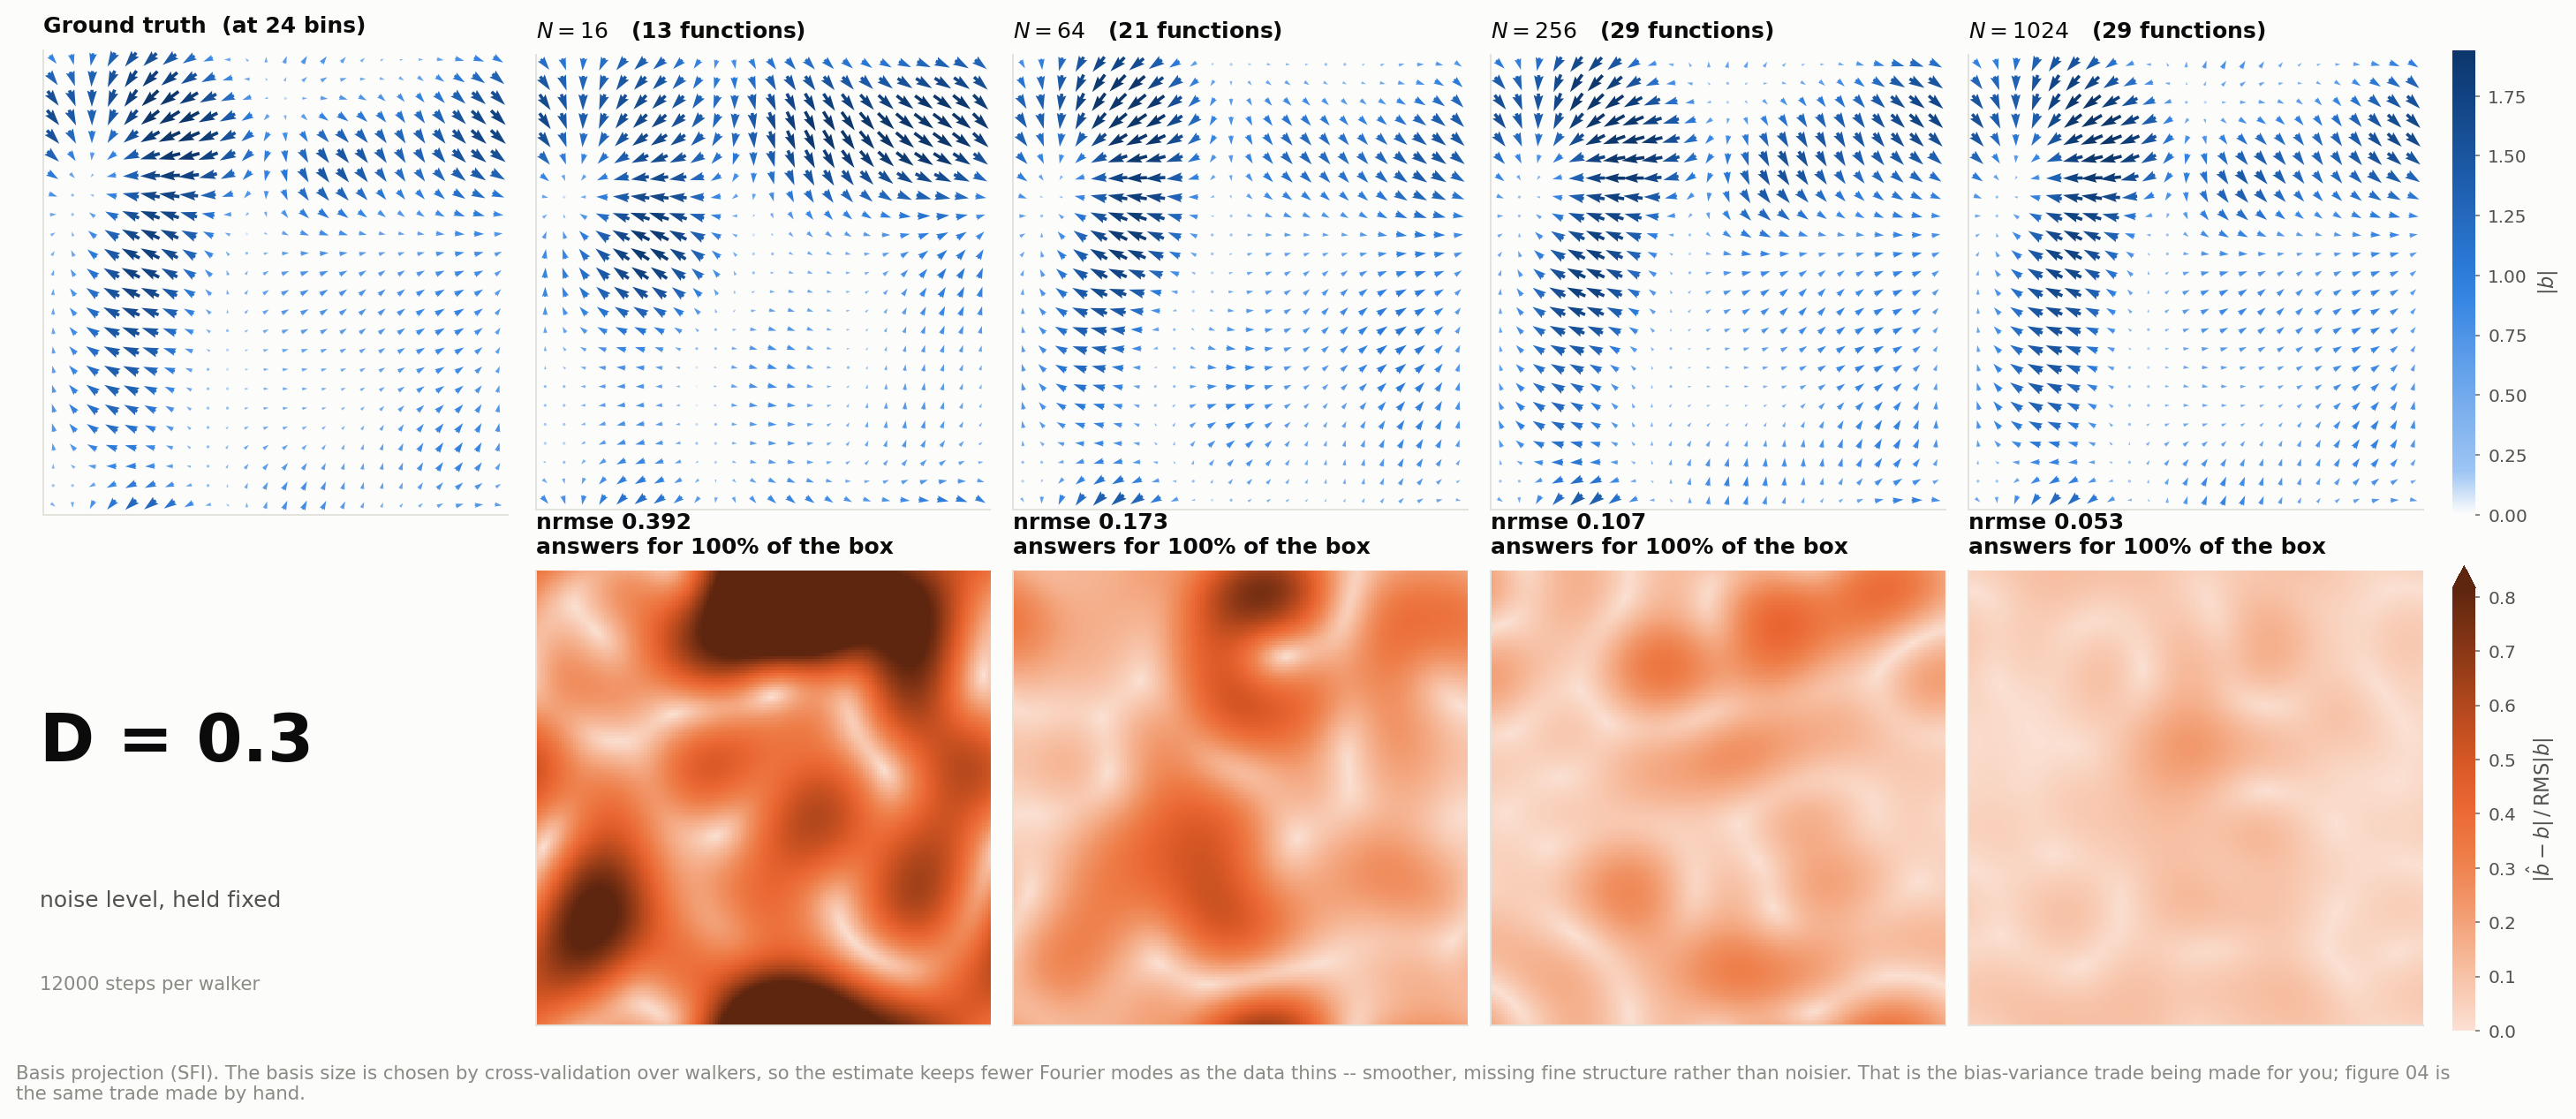
\includegraphics[width=\textwidth]{figs/recovery_vs_walkers.png}
\caption{SFI as the data grows: ground truth, then estimates from 16 to 1024 walkers, with
the error map below each. The basis size is chosen by cross-validation over walkers, so the
estimate keeps fewer modes as the data thins \textemdash{} it goes smooth and misses fine
structure rather than going noisy. Every method produces this figure on the same walkers.}
\end{figure}

\subsection{More structure beats more flexibility \textemdash{} until the structure is wrong}

In the reference column the order is binning (0.293), kernel (0.126), network (0.100),
Fourier basis (0.097). Each step buys accuracy by assuming more, and here the assumptions
happen to be true: these fields \emph{are} sums of Fourier modes, so SFI's basis is not a
convenience but a match. On fields built by other generators (sparse wells, cellular
patterns) SFI loses that edge to the kernel, which assumes only smoothness. The per-dataset
network sits in the middle almost everywhere and wins among the classical methods where data
is scarcest (0.340 at 16 walkers).

\subsection{The amortised network: a learned prior, its gain, and its price}
\label{sec:amort}

\textbf{In distribution, it wins nearly everywhere.} On 100 held-out fields from the
training generator, fitted at three budgets (median 64k, 256k and 1M transitions), its median
nrmse is 0.213, 0.122 and 0.070 against 0.334, 0.192 and 0.089 for the better of SFI and the
kernel \textemdash{} it is the better method on 99\%, 97\% and 93\% of fields. On the reference
walkers it reaches 0.060 against SFI's 0.097, without cross-validation and in 0.6 seconds.

\textbf{What it learned: a filter, not a bandwidth.} To see what the network does, linearise
it. Its output at one node $c_0$ responds to the mean increment $\bar Y_c=Y_c/N_c$ of every
cell $c$ through the \emph{equivalent kernel}
\begin{equation}
  K_c = \frac{\partial \hat b(c_0)}{\partial \bar Y_c},
  \qquad
  \hat b(c_0) \approx \sum_c K_c\,\bar Y_c ,
\end{equation}
computed exactly by automatic differentiation. Two numbers summarise it: its \emph{width}
(the RMS radius of $|K|$), and its \emph{gain} $G=\sum_c K_c$, the fraction of a uniform drift
that passes through. A classical smoother has $G=1$ by construction (its weights sum to one)
and adapts by changing its width: as data grow, the cross-validated kernel bandwidth roughly
halves, from about 0.17 to 0.08. The network does the opposite:

\begin{center}
\small
\begin{tabular}{@{}lrrrr@{\qquad}lrrrr@{}}
\toprule
walkers & 16 & 64 & 256 & 1024 & $D$ & 0.05 & 0.15 & 0.4 & 1.0 \\
\midrule
width & 0.260 & 0.259 & 0.237 & 0.262 & width & 0.119 & 0.177 & 0.256 & 0.337 \\
gain $G$ & 0.60 & 0.77 & 0.92 & 0.93 & gain $G$ & 0.79 & 0.93 & 0.76 & 0.39 \\
\bottomrule
\end{tabular}
\end{center}

As the budget grows 64-fold its width barely moves and its gain rises from 0.60 to 0.93.
As the noise grows it widens \emph{and} shrinks harder, down to $G=0.39$ at $D=1$.

\textbf{Why shrinking is the right thing to learn.} A smoother with gain 1 is unbiased but
passes all the noise it averages; multiplying the estimate by $G<1$ adds a bias $(1-G)\,b$ and
cuts the variance by $G^2$. When noise dominates, that trade is strongly favourable, and the
optimal amount of shrinkage depends on how large fields typically are \textemdash{} on the
prior. In the idealised linear-Gaussian case the Bayes-optimal estimator is the Wiener filter,
which acts on each Fourier mode $k$ of the data separately,
\begin{equation}
  \hat b(k) \;=\; \frac{S(k)}{S(k)+\mathcal N(k)}\;\bar Y(k),
\end{equation}
with $S$ the power spectrum of the field prior and $\mathcal N\propto\sigma^2/n$ the noise
power per mode. More data lowers $\mathcal N$ and pushes the factor towards 1 \textemdash{} the
gain rises; more noise raises it and suppresses the high-$k$ modes first \textemdash{} the
filter widens and shrinks. The network is not linear, and not exactly this filter, but it
shows its signature. Its kernels are also elongated with negative side lobes: the $x$-component
of a gradient field is correlated further along $y$ than along $x$, and the network learned
that anisotropic covariance, which no isotropic bandwidth can represent.

\begin{figure}[h]
\centering
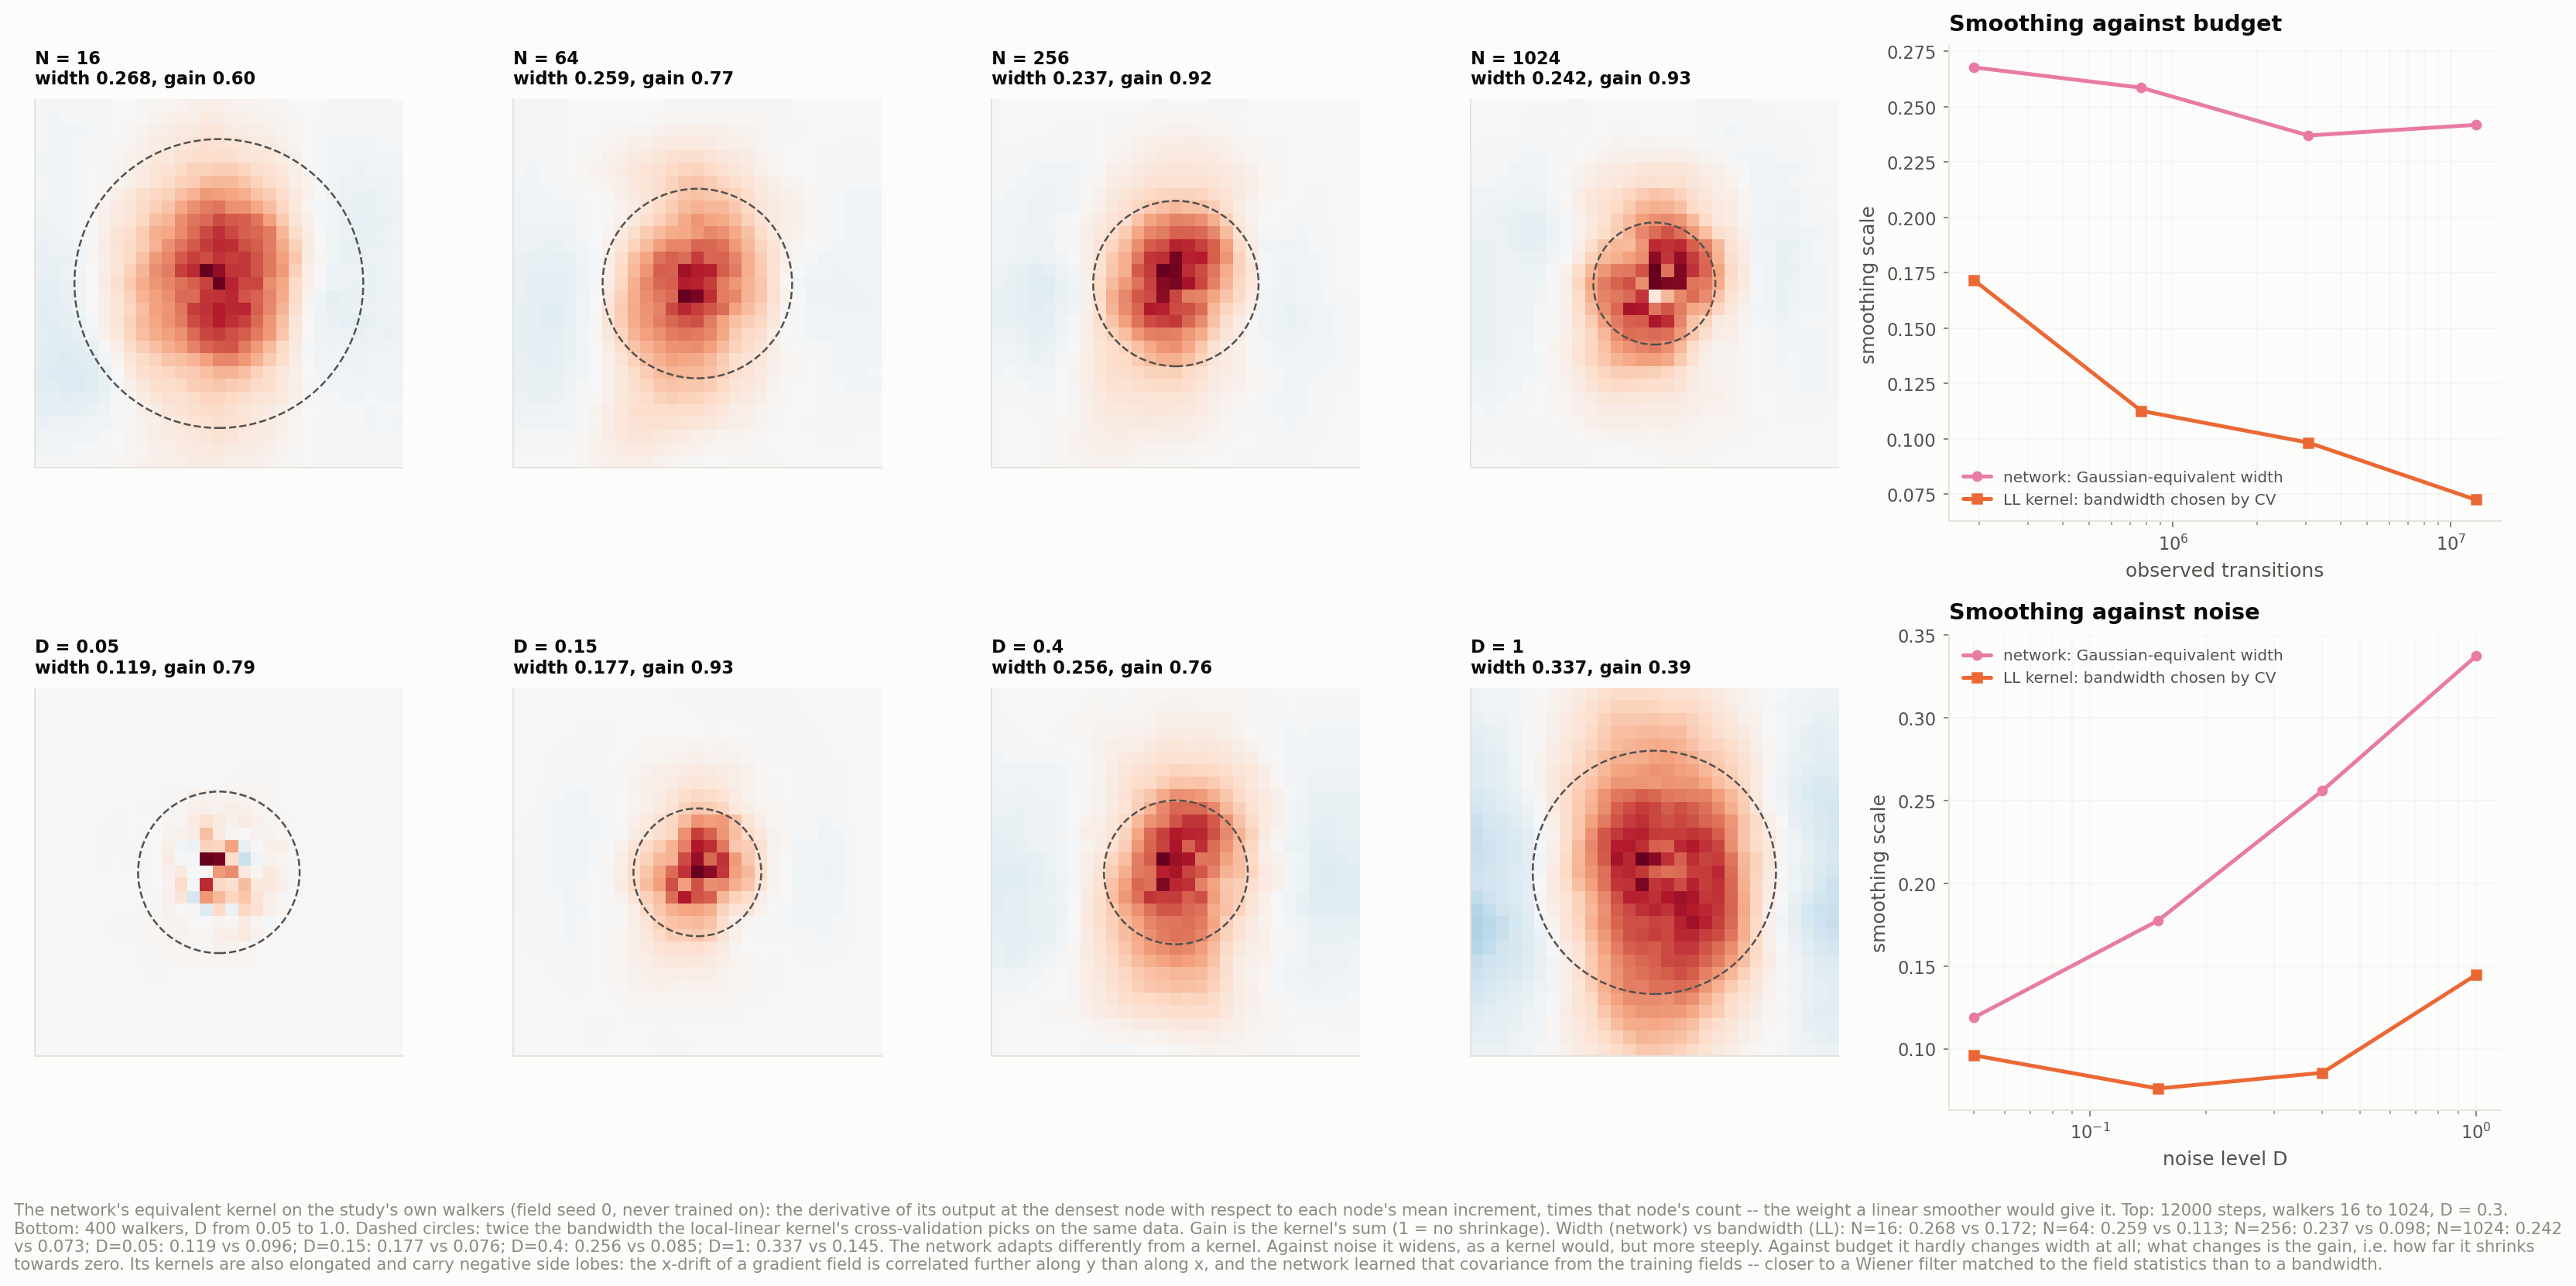
\includegraphics[width=0.95\textwidth]{figs/learned_smoothing.png}
\caption{The network's equivalent kernel $K_c$ on the reference field (never seen in
training). Top: walkers from 16 to 1024 at $D=0.3$. Bottom: $D$ from 0.05 to 1 at 400
walkers. Dashed circles: twice the bandwidth that cross-validation picks for the
local-linear kernel on the same data. Right: width against budget and against noise for both.}
\end{figure}

\textbf{The price: a prior can be wrong.} Everything above hinges on the training generator
being a good model of the field. When it is not, the bias $(1-G)\,b$ that was cheap becomes
the dominant error, because the network shrinks the features its prior considers unlikely.
On six generators it never saw (eight fields each, 1M transitions, same amplitude):

\begin{center}
\small
\begin{tabular}{@{}lrrrrrr@{}}
\toprule
median nrmse & egg carton & terraces & power-law & Perlin & band-pass & sparse wells \\
\midrule
local-linear kernel & 0.283 & \textbf{0.602} & \textbf{0.612} & \textbf{0.642} & 0.442 & 0.375 \\
SFI & 0.163 & 0.619 & 0.729 & 0.743 & \textbf{0.379} & \textbf{0.356} \\
amortised CNN & \textbf{0.151} & 0.702 & 0.726 & 0.803 & 0.721 & 0.683 \\
\emph{amortised / best} & \emph{0.92} & \emph{1.17} & \emph{1.19} & \emph{1.25} & \emph{1.90} & \emph{1.92} \\
\bottomrule
\end{tabular}
\end{center}

It wins only on the egg carton, a smooth single-scale field that resembles a long-correlation
training field. It is worst exactly where the classical methods do well. A band-pass field
concentrates its power on a ring of wavenumbers that the Gaussian prior considers improbable
at that amplitude, so those modes are damped. Sparse wells \textemdash{} a plain of zero drift
broken by narrow wells with drift up to $4\times$ the RMS \textemdash{} are treated as noise:
smoothed away and pulled back towards the amplitudes the network knows. Shifting a parameter
beyond the training range shows the same rule: a rotation $\omega=3$ (trained $|\omega|\le1.5$)
costs $3.3\times$, a drift twice as strong $2.2\times$, near-noise-free data ($D=0.02$)
$3.5\times$; but rougher fields, smoother fields and much noisier data, which the prior does
not forbid, are survived or still won. SFI and the kernel have no training distribution to
leave; their errors move only with the difficulty of the problem.

\begin{keybox}
The amortised network is better because it knows what the answer should look like, and it
degrades exactly as far as that knowledge is wrong. Use it where the training generator is a
credible model of the system; otherwise train it on a broader mix of generators.
\end{keybox}

\subsection{At equilibrium, static positions beat increments, increasingly with dimension}

On a gradient field ($\omega=0$), denoising score matching on 500k independent snapshots
reaches 0.072 in 2D, where the best per-dataset trajectory method on 4.8M increments gets
0.097. Using the walkers' own (time-correlated) positions instead of idealised snapshots, it
still beats every per-dataset trajectory method at 16 and 64 walkers (0.302 and 0.164,
against 0.340 and 0.173 for the best of them). The advantage grows with dimension:

\begin{center}
\small
\begin{tabular}{@{}lrrrr@{\qquad}lrrrr@{}}
\toprule
\multicolumn{5}{@{}l}{\textit{trajectories, 6.1M transitions}} & \multicolumn{5}{l@{}}{\textit{snapshots, up to 500k positions}} \\
& $d=2$ & 3 & 5 & 10 & & $d=2$ & 3 & 5 & 10 \\
\midrule
SFI & 0.082 & 0.195 & 0.946 & 1.002 & KDE score & 0.128 & 0.231 & 0.983 & 0.997 \\
local-linear & 0.116 & 0.261 & 0.925 & 1.004 & DSM & \textbf{0.072} & \textbf{0.142} & \textbf{0.625} & 0.996 \\
MLP & 0.093 & 0.223 & 0.927 & 1.019 & & & & & \\
\bottomrule
\end{tabular}
\end{center}

At $d=5$ every trajectory method sits near 0.93, barely better than predicting zero, while
denoising score matching reaches 0.625 \textemdash{} from twelve times fewer samples. Three
things explain it.

\textbf{Increments lose information as $d$ grows; positions do not.} Information about $b$
accumulates with observed \emph{time}, not with the number of steps: the variance of a local
estimate is $2D/T_{\mathrm{occ}}$, with $T_{\mathrm{occ}}$ the time spent in the region (§5).
A stable simulation needs $\dt$ to shrink with $d$ (the diffusive step $\sqrt{2dD\dt}$ must
stay small against the field's length scale): $\dt=1.05\times10^{-3}$ in 2D but
$2.7\times10^{-4}$ in 5D. The same 6.1M transitions therefore cover four times less time,
and the per-step noise grows from 32 to 109 times the drift. Meanwhile the field has
${\sim}1700$ independent correlation volumes in 5D. The 1600 time units of data leave about
one unit per volume, a standard deviation $\sqrt{2D}\approx0.8$ per component against a
signal of 0.44: below one in signal-to-noise everywhere, which is why every trajectory
method retreats towards zero. Not capacity \textemdash{} the same MLP fits the exact 5D drift
to 0.04 given noiseless targets \textemdash{} but information.

\textbf{A snapshot is a full, independent sample.} Each position is a draw from $\rss$, whose
log-gradient \emph{is} the drift (divided by $D$); its information does not depend on $\dt$
at all. 500k snapshots give ${\sim}300$ independent samples per correlation volume, and the
noise in the score regression is the noise level $\sigma$ the method chooses, not the
$\sqrt{2D/\dt}$ imposed by the physics.

\textbf{A shared model, not a local average.} The KDE score is a fixed-bandwidth local average
whose gradient variance grows like $h^{-(d+2)}$ \textemdash{} the same curse as binning, and it
fails in 5D (0.983). Denoising score matching fits one neural network across the whole
space, pooling statistical strength between regions. At $d=10$, 500k snapshots are no longer
enough for either.

This advantage lives entirely on the equilibrium side of \eqref{eq:split}: it requires
$J_{\mathrm{ss}}=0$, and it disappears with the circulation, as the next section shows.

\subsection{Snapshots are blind to circulation, exactly}

\begin{figure}[h]
\centering
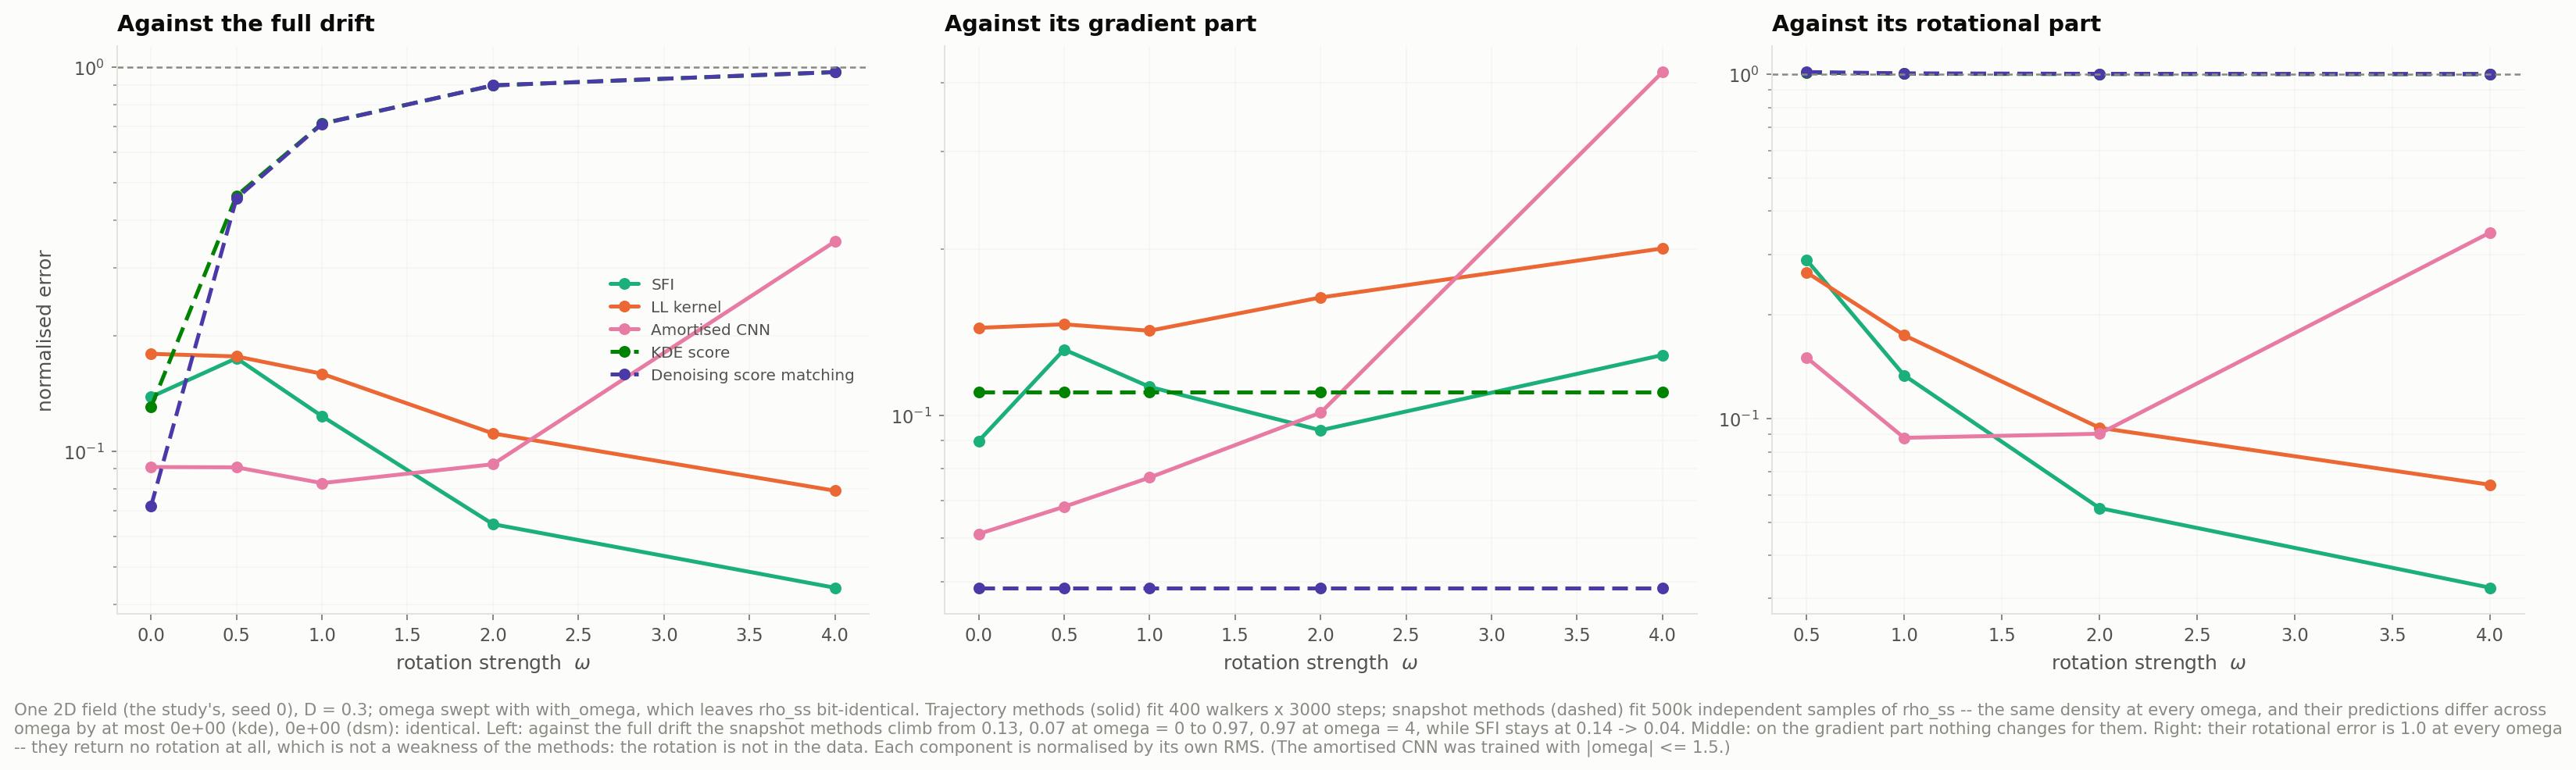
\includegraphics[width=\textwidth]{figs/identifiability_report.png}
\caption{One field with $\omega$ swept from 0 to 4, which leaves $\rss$ bit-identical. Left:
against the full drift the snapshot methods (dashed) climb towards 1 while trajectory methods
improve. Middle: against the gradient part the snapshot methods are flat. Right: against the
rotational part their error is 1.00 everywhere \textemdash{} they return no rotation at all.}
\end{figure}

As \eqref{eq:split} predicts, both snapshot estimators return \emph{bit-identical}
predictions for $\omega=0,\dots,4$ (largest difference across the five values: exactly 0.0).
Their error against the rotational component is 1.00 at every $\omega$, and against the full
drift it climbs as $\omega/\sqrt{1+\omega^2}$, the fraction of $|b|$ that is rotational.
Trajectory methods instead \emph{improve} with $\omega$: a stronger rotation is more signal
against the same noise. The amortised network tracks $\omega$ up to 2 and fails at 4,
outside its training range.

\subsection{Position measurement error: a bias for trajectories, almost nothing for snapshots}

In experiments positions are measured with error \textemdash{} for instance the localisation
error of a microscope. Model it as $\tilde x_k = x_k+\varepsilon_k$ with independent
$\varepsilon_k\sim\mathcal N(0,\sigma^2 I)$. The two families react completely differently.

\textbf{Trajectories.} The measured increment is
$\Delta\tilde x_k = \dx_k + \varepsilon_{k+1} - \varepsilon_k$. This adds variance $2\sigma^2$,
which averages out like any other noise. It also adds a \emph{bias}, which does not. Every
trajectory method groups increments by their measured starting point $\tilde x_k$, and the
same $\varepsilon_k$ that displaced that measurement enters the increment with the opposite
sign. Suppose $\rss$ increases to the right. A particle measured at $\tilde x$ is more likely
to truly sit to its right, where there are more particles, so the error
$\varepsilon_k=\tilde x_k-x_k$ tends to point left; precisely, for small $\sigma$ (Tweedie's
formula),
\begin{equation}
  \E[\varepsilon_k \,|\, \tilde x_k] \;=\; -\sigma^2\,\nabla\log\rss(\tilde x_k).
\end{equation}
The increment carries $-\varepsilon_k$, which therefore points right, towards higher density
\textemdash{} along $b$. Dividing by $\dt$ and using $\nabla\log\rss=b/D$:
\begin{equation}
  \E\Big[\frac{\Delta\tilde x_k}{\dt}\,\Big|\,\tilde x_k\Big]
  \;\approx\; b + \frac{\sigma^2}{\dt}\,\nabla\log\rss
  \;=\; b\,\Big(1+\frac{\sigma^2}{D\dt}\Big).
\end{equation}
Every trajectory method then estimates a field that is too large by this factor, however much
data it has. The ratio compares the measurement error $\sigma$ with the size of one diffusive
step $\sqrt{2D\dt}\approx0.025$: at $\sigma=0.02$, one percent of the box, they are
comparable, and the estimate is $2.3\times$ too large. Recording less often (larger $\dt$)
helps; more data does not.

\textbf{Snapshots.} Noisy positions are exact samples of the blurred density
$\rss*\mathcal N(0,\sigma^2I)$, whose score differs from the true one by a relative amount of
order $(\sigma/\ell)^2\approx10^{-2}$, with $\ell\approx0.24$ the length scale of the field.

\begin{center}
\small
\begin{tabular}{@{}lrrrr@{}}
\toprule
$\sigma_{\mathrm{obs}}$ & 0 & 0.005 & 0.01 & 0.02 \\
\midrule
predicted inflation $1+\sigma^2/(D\dt)$ & 1 & 1.08 & 1.33 & 2.31 \\
\midrule
binned & 0.473 & 0.499 & 0.662 & 1.562 \\
local-linear kernel & 0.222 & 0.220 & 0.350 & 1.246 \\
SFI & 0.200 & 0.237 & 0.439 & 1.431 \\
MLP & 0.212 & 0.238 & 0.422 & 1.379 \\
amortised CNN & 0.140 & 0.153 & 0.240 & 0.627 \\
\midrule
KDE score & 0.135 & 0.136 & 0.137 & 0.140 \\
denoising score matching & 0.077 & 0.077 & 0.078 & 0.080 \\
\bottomrule
\end{tabular}
\end{center}
{\footnotesize\color{ink2} nrmse, 256 walkers $\times$ 4000 steps, $D=0.3$, mean of 3 seeds.}

The trajectory errors track the predicted inflation: an estimate $2.3\times$ too large has an
nrmse of at least 1.3 from the bias alone, and the classical methods land between 1.25 and
1.56. The amortised network suffers less only by accident: its amplitude prior pulls the
inflated estimate back towards field magnitudes it has seen. The snapshot methods barely
move. The full derivation, verified against simulation term by term, is in the companion note
\code{docs/binned\_km\_error\_analysis.pdf}.

\subsection{Every method that tunes itself can be fooled by its own criterion}
\label{sec:selftuning}

Four instances, each caught only by comparing against the truth. Cross-validation chose a
$10^6$-cell grid that answered for 10\% of the box (binning). Early stopping quit 30\% early on
a flat held-out curve (MLP). The KDE bandwidth search ran to the bottom of its grid on
temporally correlated positions (1.06 against 0.35 at a fixed bandwidth), because it split
samples at random rather than by walker; and to the \emph{top} at $D=1$, where the density is
nearly flat and the criterion has almost no signal \textemdash{} the 0.843 in the table. Every
method therefore reports what it chose, not only what it scored.

% ==========================================================================
\section{The error budget, in closed form}

For binning the whole error decomposes analytically, and each term was verified against
simulation. For a cell of width $h$ holding $n$ increments,
\begin{equation}
  \mathrm{MSE} \;\simeq\; \underbrace{\frac{2D}{n\dt}}_{\text{variance}}
  \;+\;\underbrace{\frac{|\nabla b|^2h^2}{12}}_{\text{bias: one value per cell}}
  \;+\;\underbrace{b^2\Big(\frac{\sigma_{\mathrm{obs}}^2}{D\dt}\Big)^{\!2}}_{\text{bias: position error}},
  \qquad n \simeq M\rss h^d ,
\end{equation}
with $M$ the total number of transitions. Substituting $n$ gives three facts that govern
every trajectory method:
\begin{itemize}[leftmargin=1.2em,itemsep=0.1em]
\item $\mathrm{Var}=2D/(M\rss h^d\dt)=2D/T_{\mathrm{occ}}$ depends only on the \emph{time}
      spent in the cell. Sampling faster makes each $\dx/\dt$ noisier and gives
      proportionally more of them: $\dt$ cancels.
\item Balancing variance against bias gives $h^\star\propto M^{-1/(d+2)}$ and
      $\mathrm{MSE}^\star\propto M^{-2/(d+2)}$: to halve the error at $d=6$ takes $16\times$ the
      data. This is the basic reason to go beyond binning.
\item The position-error term keeps its $1/\dt$, so with imperfect measurements sampling
      faster is actively harmful.
\end{itemize}
Against 64 independent simulated replicas: the variance law holds to within
1\textendash9\% at every cell width and local density, the predicted optimal bin count is 17.0
against a measured 16, and the inflation factor is confirmed to 1.5\%.

% ==========================================================================
\section{Limitations}

\begin{itemize}[leftmargin=1.2em,itemsep=0.12em]
\item \textbf{The families are not compared like for like.} The amortised network knows the
      field distribution; the snapshot methods get independent samples and the true $D$.
\item \textbf{One field family, one box.} Almost every number comes from Gaussian-spectrum
      fields on $[-1,1]^2$; the other-generator test is the only breadth check, and it is 2D.
\item \textbf{$D$ is known} to the snapshot methods, and $\dt$ is set by the simulator's
      stability rule rather than by an experiment.
\item \textbf{The snapshot estimators receive positions without walker labels}, so their
      cross-validation cannot group by walker. That is a real defect when positions are
      correlated in time.
\item \textbf{The amortised network is 2D-only}, and its $64^2$ output grid caps its accuracy
      on nearly noise-free data.
\end{itemize}

% ==========================================================================
\section{What is worth doing next}

\begin{enumerate}[leftmargin=1.4em,itemsep=0.12em]
\item \textbf{A hybrid estimator}: the gradient part from positions, the rotational remainder
      from increments. With few walkers it should beat both families.
\item \textbf{Estimate $D$ from the data} (quadratic variation) in the snapshot methods and
      report how the drift scale degrades.
\item \textbf{Train the amortised network on a mixture of generators} and repeat the test
      above; how much in-family accuracy it trades for robustness is the interesting number.
\item \textbf{A calibrated posterior}: a conditional diffusion model over drift fields giving
      a distribution rather than a point estimate, with coverage checked against the truth.
\item \textbf{A time-resolution sweep}, where the error budget predicts the $O(\dt)$
      discretisation bias trading against the $1/\dt$ measurement-error amplification.
\item \textbf{Real data} \textemdash{} single-particle tracking or an ecological time series:
      unknown $D$, non-stationary boundaries, heterogeneous noise.
\end{enumerate}

% ==========================================================================
\section{Reproducing this}

Every figure and table comes from a numbered script: \code{01} (fields and trajectories),
\code{03} (the six shared figures for every method), \code{04} (kernel against binning),
\code{05}\textendash\code{07} (amortised network: data, training, study), \code{08} (snapshot
methods and identifiability), \code{09} (the error budget); \code{python -m pytest tests/} runs
the 46 tests. Result tables are cached by configuration in \code{outputs/*/data/}, so a re-run
redraws the figures without recomputing anything. Per-method detail is in the
\code{README.md} of each folder under \code{outputs/}, the cross-method comparison in
\code{outputs/SUMMARY.md}, and the framework reference and the analytical note in
\code{docs/}.

\end{document}
